
\documentclass[10 pt,usenames,dvipsnames, oneside]{article}
\usepackage{../../modelo-fracoes}
\graphicspath{{../../../Figuras/licao04/}}


\begin{document}

\begin{center}
  \begin{minipage}[l]{3cm}

\includegraphics[width=2cm]{../../../Figuras/logo}       
\end{minipage}\hfill
\begin{minipage}[r]{.8\textwidth}
 {\Large \scshape Atividade: Marcações nos copos cilíndricos}  
\end{minipage}
\end{center}
\vspace{.2cm}

\ifdefined\prof
%Caixa do Para o Professor
\begin{goals}
%Objetivos específicos
\begin{enumerate}
    \item       Usar igualdade de frações para calcular o numerador de uma das
frações em uma situação contextualizada.
\end{enumerate}

\tcblower

%Orientações e sugestões
\begin{itemize}
    \item       Recomenda-se que, nesta atividade, os alunos trabalhem
individualmente ou em duplas. No entanto, é fundamental que os alunos sejam
estimulados a explicar o raciocínio realizado.
\end{itemize}
\end{goals}

\bigskip
\begin{center}
{\large \scshape Atividade}
\end{center}
\fi

Você tem um copo cilíndrico graduado com cinco marcas horizontais igualmente espaçadas. O copo tem suco de laranja até $\dfrac{3}{4}$ de sua capacidade, como ilustra a imagem:

\begin{center}

 \begin{tikzpicture}[scale=0.5, x=1cm,y=1cm]

% Definição do eixo vertical das elipses
\def\EixoM{0.3}

% colorindo o primeiro cilindro
\fill[light, opacity=1] (2,0) ellipse (2 and \EixoM);
\fill[light,fill opacity=.8] (0,0) rectangle (4,3);
\fill[fill=light,fill opacity=1] (2,3) ellipse (2 and \EixoM);

\pgfpathmoveto{\pgfpoint{0 cm}{0 cm}}
\pgfpatharc{-180}{0}{2cm and \EixoM cm}
\pgfusepath{draw}

\draw (2,4) ellipse (2 and \EixoM);
\draw (0,0) -- (0,4);
\draw (4,0) -- (4,4);

% shift vertical nos arcos de elipse definido por \y
\pgfsetlinewidth{2*\pgflinewidth}
\foreach \y in {0,...,4}{
\pgfpathmoveto{\pgfpoint{0 cm}{\y cm}}
\pgfpatharc{-180}{-130}{2cm and \EixoM cm}
\color{Green}
\pgfusepath{draw}}

\end{tikzpicture}
\end{center}

Seu colega tem um copo cilindrico idêntico, mas graduado com 17 níveis horizontais igualmente espaçados:

\begin{center}
 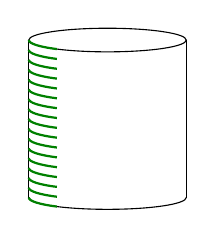
\begin{tikzpicture}[scale=0.5, x=1cm,y=1cm]

% Definição do eixo vertical das elipses
\def\EixoM{0.3}

\pgfpathmoveto{\pgfpoint{0 cm}{0 cm}}
\pgfpatharc{-180}{0}{2cm and \EixoM cm}
\pgfusepath{draw}

\draw (2,4) ellipse (2 and \EixoM);
\draw (0,0) -- (0,4);
\draw (4,0) -- (4,4);

% shift vertical nos arcos de elipse definido por \y
\pgfsetlinewidth{2*\pgflinewidth}
\foreach \y in {0,.25,...,4}{
\pgfpathmoveto{\pgfpoint{0 cm}{\y cm}}
\pgfpatharc{-180}{-130}{2cm and \EixoM cm}
\color{Green}
\pgfusepath{draw}}

\end{tikzpicture}
\end{center}

Verifique se é possível completar um número inteiro de níveis do copo de seu colega de modo a ficar com a mesma quantidade de suco. Em caso afirmativo, explique sua resposta.

\ifdefined\prof
\begin{solucao}

As 17 marcações no copo do seu colega divide a capacidade do copo em 16 partes
iguais. Quantas destas partes correspondem a   $\dfrac{3}{4}$   da capacidade do
copo (que é fração da capacidade do copo que está preenchida com suco)? Para
responder a esta pergunta, devemos calcular o numerador de uma fração de
denominador 16 que seja igual a   $\dfrac{3}{4}$  , isto é, devemos preencher
$\square$   com um número tal que

  $\dfrac{3}{4} = \dfrac{\square}{16}$.

  Como   $16 = 4 \times 4$  , segue-se que

  $\dfrac{3}{4} = \dfrac{4 \times 3}{4 \times 4} = \dfrac{12}{16}$.

  Assim, não necessárias   $12$   partes de   $\dfrac{1}{16}$   da capacidade do
copo. Consequentemente,
  13 níveis do copo do seu colega devem ser preenchidos com suco de laranja para
que ele fique com a mesma quantidade suco de laranja que você.


\begin{center}
 \begin{tikzpicture}[scale=0.5, x=1cm,y=1cm]

% Definição do eixo vertical das elipses
\def\EixoM{0.3}

% colorindo o primeiro cilindro
\fill[light, opacity=1] (2,0) ellipse (2 and \EixoM);
\fill[light,fill opacity=.8] (0,0) rectangle (4,3);
\fill[fill=light,fill opacity=1] (2,3) ellipse (2 and \EixoM);


\pgfpathmoveto{\pgfpoint{0 cm}{0 cm}}
\pgfpatharc{-180}{0}{2cm and \EixoM cm}
\pgfusepath{draw}

\draw (2,4) ellipse (2 and \EixoM);
\draw (0,0) -- (0,4);
\draw (4,0) -- (4,4);

% shift vertical nos arcos de elipse definido por \y
\foreach \y in {0,.25,...,4}{
\pgfpathmoveto{\pgfpoint{0 cm}{\y cm}}
\pgfpatharc{-180}{-130}{2cm and \EixoM cm}
\color{Green}
\pgfusepath{draw}}
\end{tikzpicture}
\end{center}

\end{solucao}
\fi

\end{document}